\subsection{Magnetohydrodynamic shock wave}
In the magnetohydrodynamic case the same initial conditions were used as for the hydrodynamic one.
A uniform magnetic field in the $x$-direction was added. 
To see the effect of the magnetic field, the simulations were carried out for the following values for the plasma-$\beta$: $\beta \in \{0.1, 0.5,1,10\}$.
This is the dimensionless $\beta$ as given by \cref{eq:plasma-beta}.
Figure \ref{fig:MHD-blasts} shows a snapshot of the blast wave at $t=0.75$ for these different values.

\begin{figure}[H]
	%\hspace{-1cm}
	\centering
	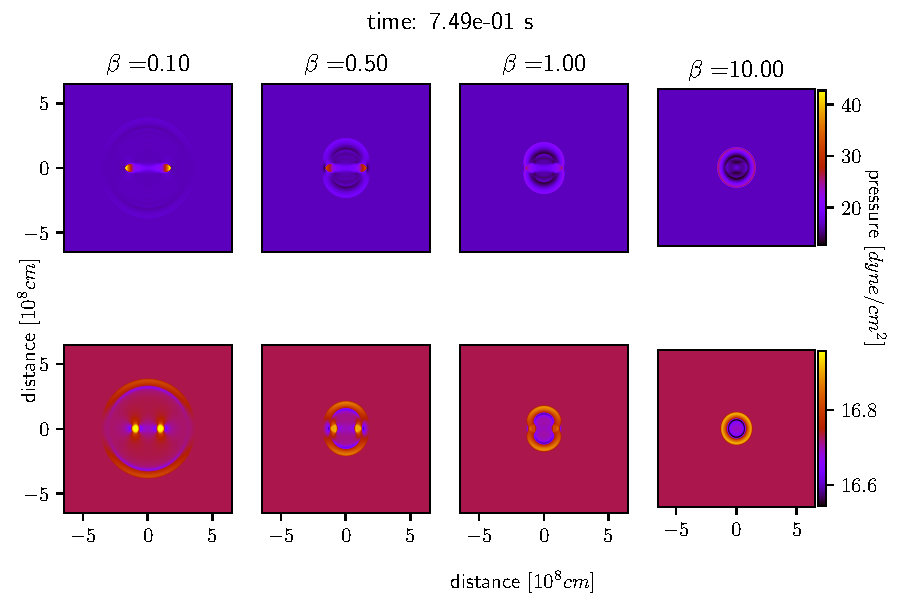
\includegraphics[width=\linewidth]{images/MHD-blasts.pdf}
	\caption{Plots of the pressure of an MHD blastwave with the same initial conditions as in \cref{fig:HD-blast-short}: high pressure difference for the top row, lower for the bottom row.
	The black circle in the middle represents the region of higher pressure in the initial condition.}
	\label{fig:MHD-blasts}
\end{figure}

The simulations for the MHD blastwave used a larger domain: 12 by 12 in code units.
This allows us to study the waves at later times when the non-linear effects have diminished because of the lower intensity of the wave.
Now we can compare these results to the linear MHD theory from \cref{sec:MHD-waves}.
The results of the simulation at earlier times can be used to compare the behaviour of an MHD shock to an HD shock.

In the plots with $\beta \in \{0.5,1\}$ there is a clear distinction between a fast shock wave spreading in all directions, and two smaller waves following the magnetic field.
In the plot with $\beta=0.1$, this fast wave is barely visible closer to the edge of the domain. In contrast, the two small waves stand out from the uniform background.
For $\beta=10$, the fast wave is almost perfectly spherical and clearly visible, whereas the two smaller waves are quite faint.
We observe that if the magnetic field is stronger, the fast wave speeds up even further, therefore fading faster because the energy in the wave is spread out more quickly.
Meanwhile the energy in the slow mode stays concentrated in a small region.
At higher magnetic field strengths the slow mode gets considerably more energetic as well.
To go a bit more in-depth, we plotted the diagram depicting the different group speeds to see how well they match. 
This can be seen in \cref{fig:MHD-group1} and \cref{fig:MHD-group2}, where the pressure profiles of the waves are plotted at $t=1.25$.
The white dashed lines show the group speed of the fast mode, the grey solid lines the group speed of the slow mode. 
The black circle is again the region with higher pressure in the initial condition.
The group speed diagram was scaled such that the curve for the fast mode would match with the fast wave mode.

\begin{figure}[H]
	%\hspace{-1cm}
	\centering
	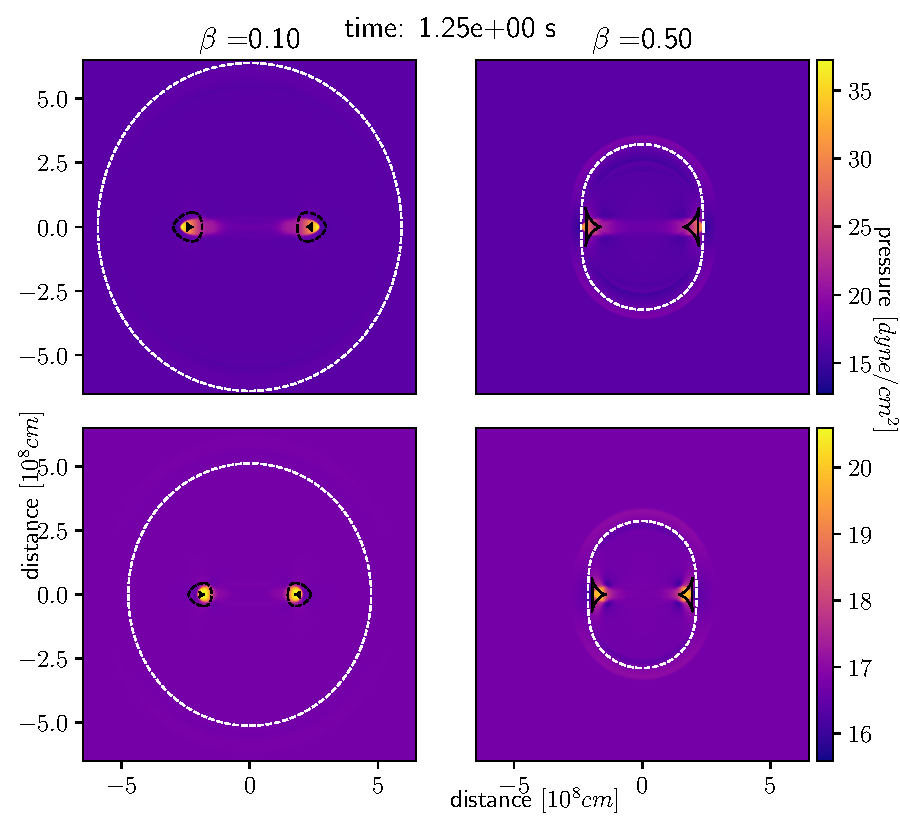
\includegraphics[width=\linewidth]{images/group-speed-pressure1.pdf}
	\caption{Plots of the pressure wave after $1.25$ time units for different values of $\beta$. 
	The white dotted line represents the theoretical position of the fast-mode magnetosonic wave.    		The grey solid lines are the parts of the group speed diagram corresponding to the slow-mode magnetosonic wave.
	The black circle in the center is the region where the pressure is higher in the initial condition.
	The top row are plots for simulations where $p_{in}=5$ at $t=0$, the bottom row simulations with $p_{in}=1.05$.}
	\label{fig:MHD-group1}
\end{figure}

Since the initial condition is not a delta function but a circle with finite radius, we cannot expect a perfect match with the theoretical group speed for linear waves.
Instead, a linear wave will be smeared out around the curves for the group speed, as if they were painted with a large brush.
Furthermore, when the pressure difference is higher, the non-linear effects will become stronger, leading to deviations from the linear theory.

In figure \cref{fig:MHD-group1}, the two scenarios with a strong magnetic field are shown (low $\beta$).
The effects of the magnetic field are again very clear, removing the isotropy by deforming the fast magnetosolic wave front, and most strikingly, introducing the slow-mode waves following the magnetic field.
Because the slow magnetosonic wave mode only travels along the field lines, its energy remains concentrated. This is the main cause of the large difference in amplitude between the slow- and fast-mode.
When the pressure difference is high, the non-linear effects stay important. 
This causes the slow mode waves in the top row in \cref{fig:MHD-group1} to travel significantly faster than linear slow wavemode.
This can be seen by notig that the yellow or red spots with high pressure are further away from the center than the grey lines denoting the theoretical group speed of the slow wavemode in the top row of \cref{fig:MHD-group1}.
In the bottom row, where the pressure difference is a lot smaller, the results match strikingly well to the linear theory.

\begin{figure}[H]
	%\hspace{-1cm}
	\centering
	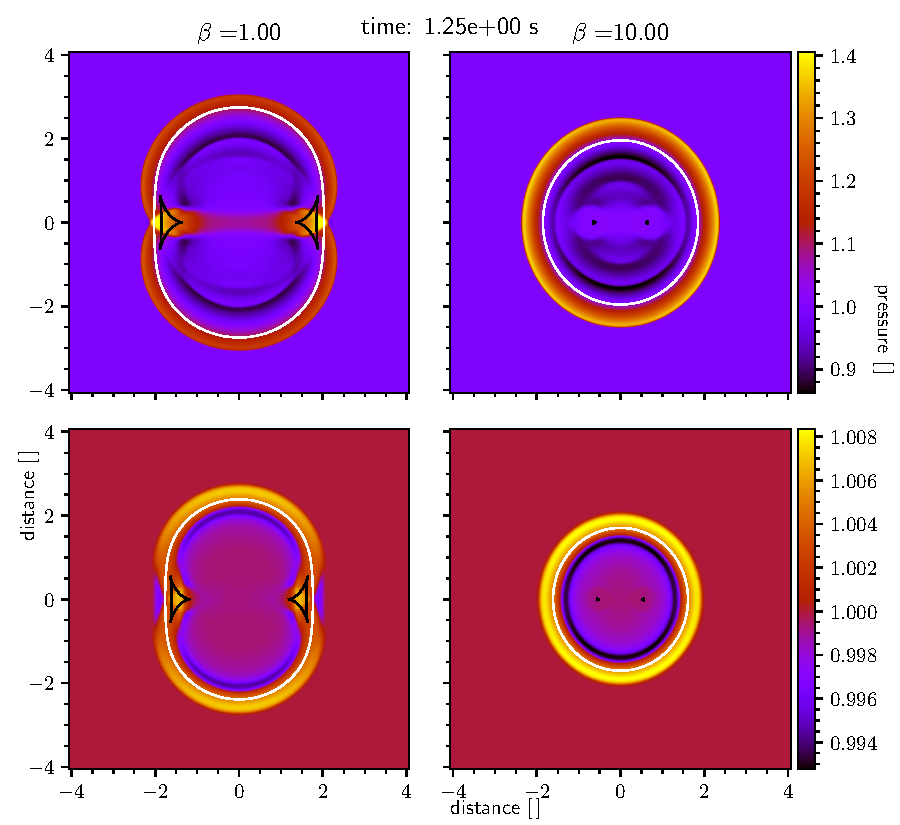
\includegraphics[width=\linewidth]{images/group-speed-pressure2.pdf}
	\caption{Same as \cref{fig:MHD-group1} but for different $\beta$ values.}
	\label{fig:MHD-group2}
\end{figure}

We also see again that the wave is faster with a higher pressure difference, like with the HD shock waves. 
Due to the difficulties in accurately detecting the waves in the simulation data, either because they are really faint with small or large $\beta$, or because there is a lot of interference between the modes when $\beta \sim 1$, no accurate calculations of the wave speed from the simulation data could be made.

When the magnetic field's strength becomes small, a quick comparison shows that the wave speed goes to the wave speed of an HD-wave, as expected.
This can be seen by comparing the rightmost graphs in \cref{fig:MHD-group2} with the rightmost graphs in \cref{fig:HD-blast-long}

